\section{Hasil dan Pembahasan}

%=========================================================%
%               TULIS ISI PEMBAHASAN DI SINI              %
% Jangan Lupa untuk Menghapus Contoh Tulisan di Bawah Ini %
%=========================================================%

Hasil pemeriksaan distribusi data pada data pelayanan kesesuaian waktu terbit perizinan dan persepsi atau penilaian konsumen terhadap layanan yang di berikan di MPP ``Grha Tiyasa'' Kota Bogor disajikan pada \autoref{fig:plot-norm-pelayanan}, \autoref{fig:plot-norm-layanan-oktober}, \autoref{fig:plot-norm-layanan-november}, dan  \autoref{fig:plot-norm-layanan-desember}. \autoref{fig:plot-norm-pelayanan} menunjukkan \textit{plot} peluang normal pada data pelayanan kesesuaian waktu terbit perizinan di MPP ``Grha Tiyasa''. Hasil \textit{output} Minitab 16.0 memberikan nilai statistik \textit{Mean}: 82,94, \textit{Standard deviation}: 22,33, nilai uji Anderson Darling: 5,701 dan \textit{p-value}: < 0,005 (lebih kecil dari tingkat signifikansi, $\alpha = 0{,}05$). Hal ini menunjukkan bahwa data tidak berdistribusi normal. Adapun rumus \textit{p-value} = $2 \times P\left( \mathrm{TS} \geq |\mathrm{ts}| \;\vert\; H_0 \text{ is true} \right) = 2 \times \left(1 - \mathrm{cdf}\left(|\mathrm{ts}|\right) \right)$ dengan:

\begin{tabbing}
    $P$ \; \= = Peluang atau probabilitas suatu kejadian \\
    TS \> = \textit{Test statistics} (uji statistik yang digunakan) \\
    ts \> = Nilai uji statistik dari sampel \\
    cdf \> = \textit{Cummulative distribution function} (fungsi distribusi kumulatif)
\end{tabbing}

\begin{figure}[H]
    \centering
    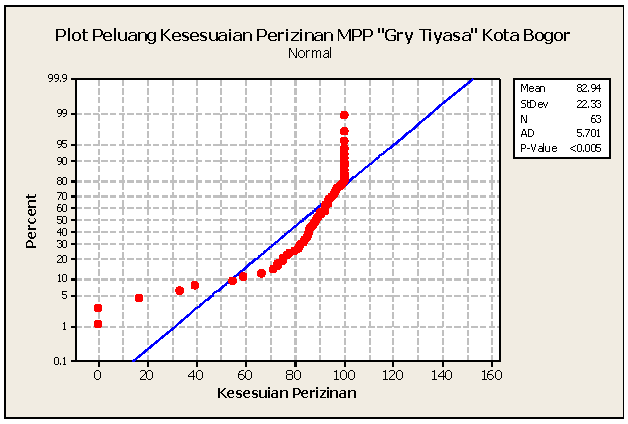
\includegraphics[width=.7\linewidth]{pdf/Plot-peluang-normal-kesesuaian-waktu-terbit-perizinan.pdf}
    \longcaption{\textit{Plot} Peluang Normal pada Pelayanan Kesesuaian Waktu \\ Terbit Perizinan}
    \label{fig:plot-norm-pelayanan}
\end{figure}

\autoref{fig:plot-norm-layanan-oktober} menunjukkan plot peluang normal persepsi konsumen pada bulan Oktober. \autoref{fig:plot-norm-layanan-oktober} menunjukkan bahwa data persepsi konsumen pada bulan Oktober berdistribusi normal. Hal ini dapat ditunjukkan dari nilai Anderson Darling: 0,566 dan \textit{p-value}: 0,101 (lebih besar dari tingkat signifikansi, $\alpha = 0{,}05$)

\begin{figure}[H]
    \centering
    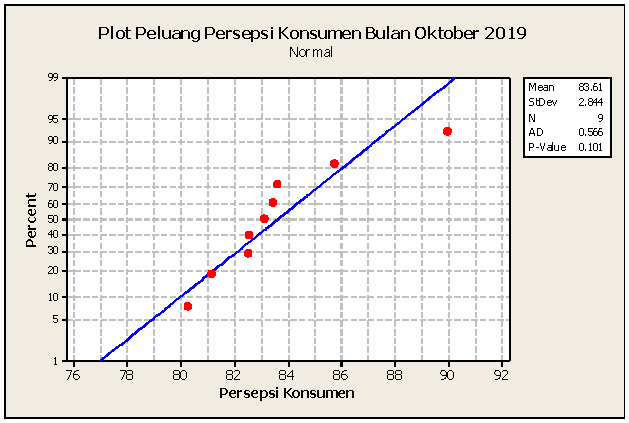
\includegraphics[width=.7\linewidth]{pdf/Plot-peluang-normal-pada-persepsi-konsumen-terhadap-layanan-di-MMP-Grha-Tiyasa-pada-bulan-Oktober-2019.pdf}
    \longcaption{\textit{Plot} Peluang Normal pada Persepsi Konsumen terhadap \\ Layanan di MPP ``Grha Tiyasa'' pada Bulan Oktober \\ 2019}
    \label{fig:plot-norm-layanan-oktober}
\end{figure}

Namun berbeda pada bulan November dan Desember. Data persepsi konsumen pada kedua bulan tersebut tidak berdistrbusi normal (\autoref{fig:plot-norm-layanan-november} dan \autoref{fig:plot-norm-layanan-desember}). Hal ini ditunjukkan oleh nilai Anderson Darling masing-masing: 0,968 dan 0,992 dengan \textit{p-value} masing-masing: 0,008 dan 0,007 (lebih kecil dari tingkat signifikansi, $\alpha = 0{,}05$). 

\begin{figure}[H]
    \centering
    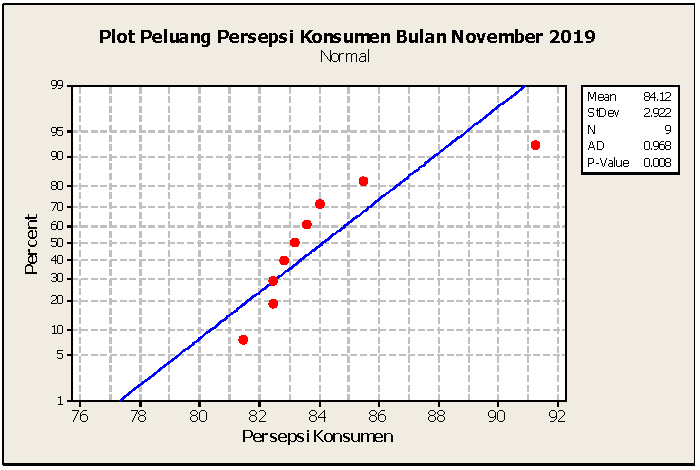
\includegraphics[width=.7\linewidth]{pdf/Plot-peluang-normal-pada-persepsi-konsumen-terhadap-layanan-di-MMP-Grha-Tiyasa-pada-bulan-November-2019.pdf}
    \longcaption{\textit{Plot} Peluang Normal pada Persepsi Konsumen terhadap \\ Layanan di MPP ``Grha Tiyasa'' pada Bulan November \\ 2019}
    \label{fig:plot-norm-layanan-november}
\end{figure}

\begin{figure}[H]
    \centering
    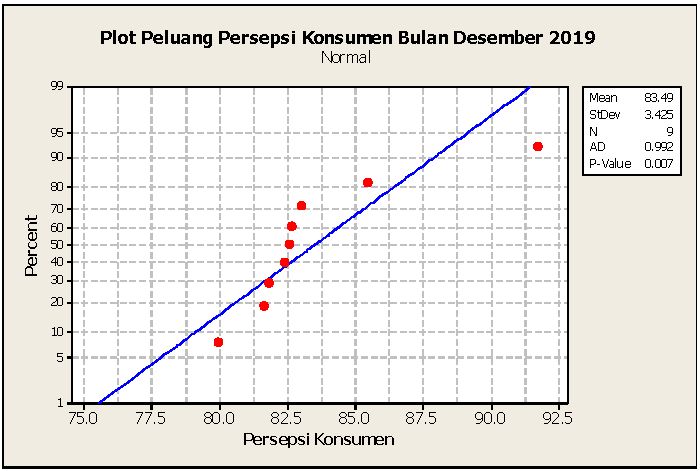
\includegraphics[width=.7\linewidth]{pdf/Plot-peluang-normal-pada-persepsi-konsumen-terhadap-layanan-di-MMP-Grha-Tiyasa-pada-bulan-Desember-2019.pdf}
    \longcaption{\textit{Plot} Peluang Normal pada Persepsi Konsumen terhadap \\ Layanan di MPP ``Gyra Tiyasa'' pada Bulan Desember \\ 2019}
    \label{fig:plot-norm-layanan-desember}
\end{figure}

Untuk keperluan analisis kapabilitas, data mengenai persepsi konsumen selama tiga bulan digabung, sehingga jika datanya digabung maka data tidak berdistribusi normal. Hal ini ditunjukkan pada \autoref{fig:plot-norm-data-persepsi} dengan nilai Anderson Darling: 2,139 dengan \textit{p-value} < 0,005 (lebih kecil dari tingkat signifikansi, $\alpha = 0,05$).

\begin{figure}[H]
    \centering
    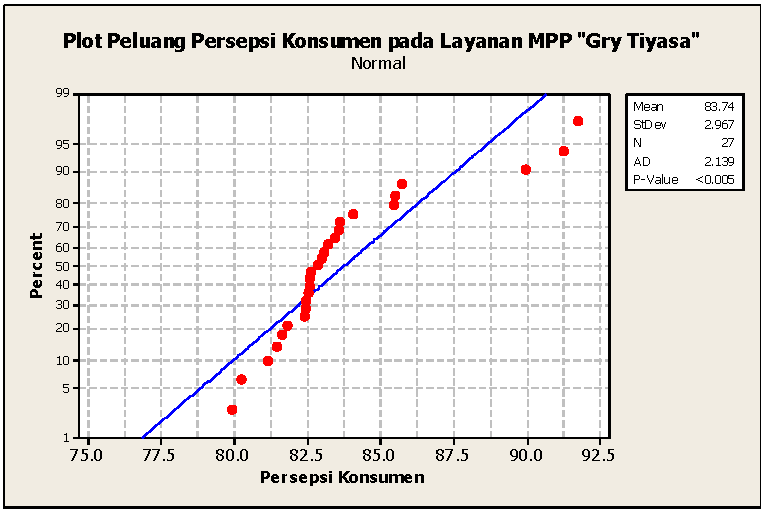
\includegraphics[width=.7\linewidth]{pdf/Plot-peluang-normal-pada-data-persepsi-konsumen-selama-3-bulan.pdf}
    \longcaption{\textit{Plot} Peluang Normal pada Data Persepsi Konsumen \\ Selama 3 Bulan}
    \label{fig:plot-norm-data-persepsi}
\end{figure}

Tahap selanjutnya dalam menentukan analisis kapabilitas proses terhadap data layanan waktu terbit perizinan. Berdasarkan hasil \textit{output} pada \autoref{fig:plot-norm-layanan-oktober}, \autoref{fig:plot-norm-layanan-november}, dan \autoref{fig:plot-norm-layanan-desember} telah ditunjukkan bahwa data tidak berdistribusi normal. Oleh karena itu, analisis kapabilitas proses menggunakan distribusi non-normal. Hasil analisis kapabilitas proses terhadap data layanan
perizinan disajikan pada \autoref{fig:kapabilitas-proses-terbit-izin}.

Dari \autoref{fig:kapabilitas-proses-terbit-izin} terlihat bahwa data layanan waktu terbit perizinan lebih mendekati distibusi Weibull dengan \textit{shape}: 175,764 dan \textit{scale}: 2092,15. Dari hasil \textit{output} Minitab 16.0 menunjukkan bahwa nilai $P_\upp = 1$, artinya kapabilitas proses dapat dikatakan sudah baik, namun masih dapat ditingkatkan kualitasnya. Selain itu, kriteria kapabilitas proses yang lain yaitu $P_{\mathrm{pk}}$. Dari hasil \textit{output} $P_{\mathrm{pk}} = 0{,}49$. Hal ini menunjukkan rata-rata dari proses dalam batas spesifikasi, tetapi sebagian dari variasi proses berada di luar batas-batas spesifikasinya. Lebih jelasnya, kondisi ini dapat digambarkan melalui \textit{I-MR Chart} pada \autoref{fig:IMRChart-proses-terbit-izin}. Dari \autoref{fig:IMRChart-proses-terbit-izin} terlihat ada dua \textit{dot} merah yang berada di luar batas spesifikasi. Dengan demikian dapat dikatakan bahwa layanan waktu terbit perizinan yang dikelola di MPP ``Grha Tiyasa'' sudah cukup baik dan memadai. Namun, MPP ``Grha Tiyasa'' dapat lebih meningkatkan lagi kualitas layanannya dengan memperhatikan jenis perizinan dan waktu berlaku perizinan yang ada.

\begin{figure}[H]
    \centering
    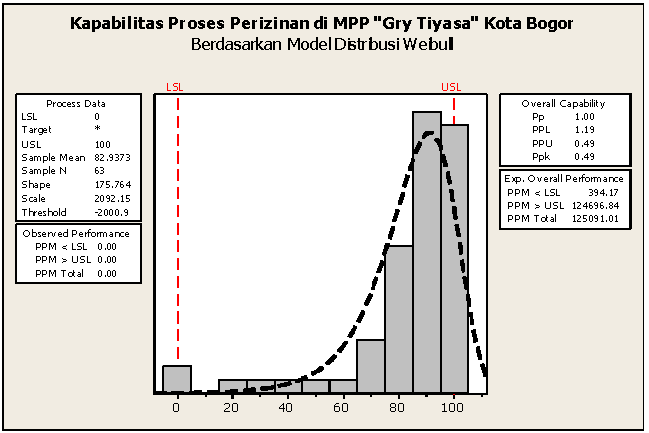
\includegraphics[width=.7\linewidth]{pdf/Analisis-kapabilitas-proses-pada-layanan-waktu-terbit-perizinan-di-MMP-Grha-Tiyasa.pdf}
    \longcaption{Analisis Kapabilitas Proses pada Layanan Waktu Terbit \\ Perizinan di MPP ``Grha Tiyasa''}
    \label{fig:kapabilitas-proses-terbit-izin}
\end{figure}

Hasil analisis kapabiltas persepsi konsumen terhadap layanan di MMP ``Grha Tiyasa'' disajikan pada \autoref{fig:kapabilitas-persepsi-layanan}. Dari \autoref{fig:kapabilitas-persepsi-layanan} terlihat bahwa data mendekati distribusi lognormal dengan \textit{location}: 4,428 dan \textit{scale}: 0,036. Dari hasil \textit{output} Minitab 16.0 menunjukkan bahwa nilai $P_\upp = 5{,}52$ artinya sebaran pengamatan atau lebar proses lebih kecil daripada lebar spesifikasi. Nilai ini mengindikasikan bahwa proses cukup baik tetapi perlu dilakukan perbaikan agar $P_\upp$ minimal 1,33 \cite{gasperz2004production}. Selain itu, dilihat dari kriteria nilai $P_{\mathrm{pk}}$ sebesar 1,70 (lebih dari 1) hal ini menunjukkan bahwa semuanya berada dalam batas spesifikasi. Kenyataan ini dapat juga dilihat pada \autoref{fig:IMRChart-persepsi-layanan}.

\begin{figure}[H]
    \centering
    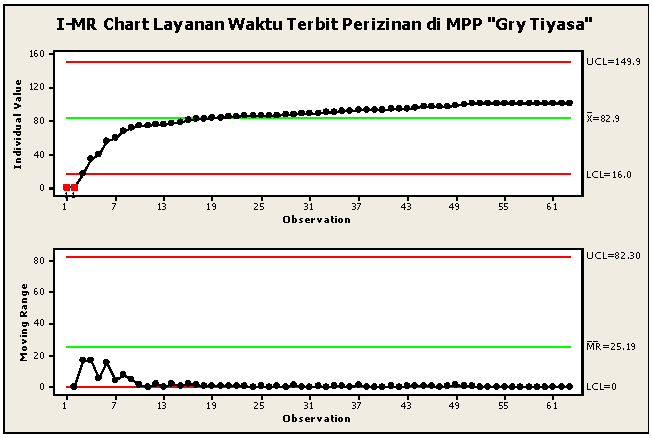
\includegraphics[width=.7\linewidth]{pdf/I-MR-chart-pada-layanan-waktu-terbit-perizinan-di-MMP-Grha-Tiyasa.pdf}
    \longcaption{\textit{I-MR Chart} pada Layanan Waktu Terbit Perizinan \\ di MPP ``Grha Tiyasa''}
    \label{fig:IMRChart-proses-terbit-izin}
\end{figure}

\begin{figure}[H]
    \centering
    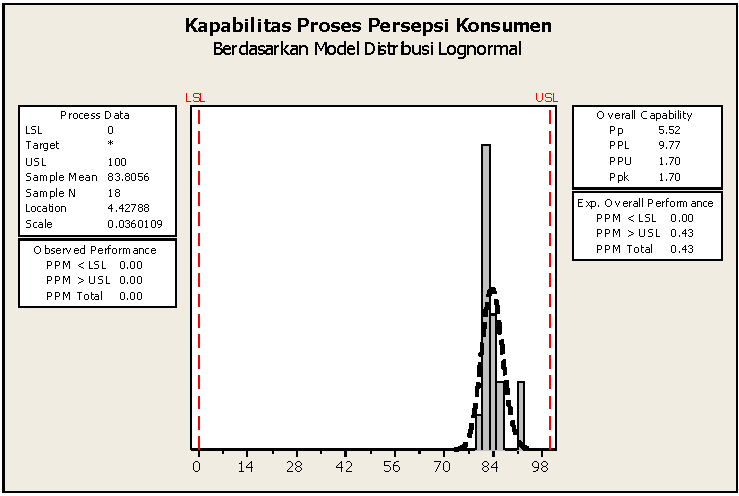
\includegraphics[width=.7\linewidth]{pdf/Analisis-kapabilitas-proses-persepsi-konsumen-terhadap-layanan-di-MMP-Grha-Tiyasa.pdf}
    \longcaption{Analisis Kapabilitas Proses Persepsi Konsumen terhadap \\ Layanan di MPP ``Grha Tiyasa''}
    \label{fig:kapabilitas-persepsi-layanan}
\end{figure}

\autoref{fig:IMRChart-persepsi-layanan} memperlihatkan bahwa kondisi hasil analisis kapabilitas yang menunjukkan semuanya berada dalam batas spesifikasi. Dari \autoref{fig:IMRChart-persepsi-layanan} terlihat bahwa tidak ada satu pun data observasi yang melebihi batas spesifikasi yang telah ditentukan.

\begin{figure}[H]
    \centering
    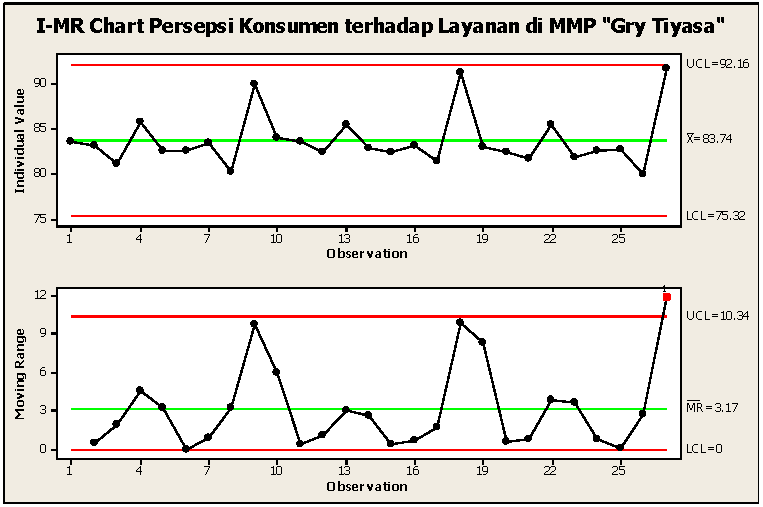
\includegraphics[width=.7\linewidth]{pdf/I-MR-chart-persepsi-konsumen-terhadap-layanan-di-MMP-Grha-Tiyasa.pdf}
    \longcaption{\textit{I-MR Chart} Persepsi Konsumen terhadap Layanan \\ di MPP ``Grha Tiyasa''}
    \label{fig:IMRChart-persepsi-layanan}
\end{figure}